\documentclass[10pt]{beamer}

\usepackage{lmodern}
\usetheme[progressbar=frametitle]{metropolis}
\usepackage{appendixnumberbeamer}
\usepackage{lipsum}
\usepackage{amsmath}
\usepackage{amssymb}
\usepackage{booktabs}
\usepackage[scale=2]{ccicons}
\usepackage{pgfplots}
\usepackage{dirtytalk}
\usepackage{xspace}
\newcommand{\themename}{\textbf{\textsc{metropolis}}\xspace}
\definecolor{mpigreen}{HTML}{007977}
\setbeamercolor{frametitle}{bg=mpigreen}

\title{DỰ ĐOÁN GIÁ CỔ PHIẾU}
\author{Giáo viên hướng dẫn: TS. Dương Hữu Phúc}
\institute{Trình bày: \\ 51704115 - Nguyễn Trung Kiều Trang
                      \\ 51703037 - Lê Thành Kiến An
                    \\ 51704071 -  Đào Nguyệt Minh}
\titlegraphic{\hfill
\includegraphics[height=1.5cm]{logoTDT.PNG}}

\begin{document}
\maketitle
\begin{frame}{NỘI DUNG}
    \begin{itemize}
        \item Ý tưởng
        \item Cấu trúc Dataset
        \item Giới thiệu thuật toán sử dụng
        \begin{itemize}
            \item Cây Quyết Định
            \item Linear
            \item Long Short Term Memory
            \item K-Means
            
        \end{itemize}
          \item Kết quả nhận được 
    \end{itemize}

\end{frame}


\begin{frame}{GIỚI THIỆU Ý TƯỞNG}
    \begin{itemize}
        \item Vì có tính thực tế cao
        \item Đầu tư linh hoạt
        \item Mọi giao dịch của bạn liên quan đến mua bán chứng khoán sẽ được thực hiện nhanh chóng
        \item Khả năng mang lại lợi nhuận cao
        \item Dễ dàng đưa ra quyết định
    \end{itemize}
\end{frame}

\begin{frame}{Cấu Trúc Dataset}
\begin{itemize}
    \item Có 8 thuộc tính trong Dataset:
    \begin{itemize}
        \item Date: Ngày thưc hiện giao dịch (cấu trúc: dd - mm - yyyy
        \item Open: Giá cổ phiếu khởi điểm (cấu trúc: float)
        \item Close: Giá cổ phiếu giao dịch sau 1 ngày (cấu trúc: float)
        \item High: giá cổ phiếu cao nhất trong ngày (cấu trúc: float)
        \item Low: Giá cổ phiếu thấp nhất trong ngày (cấu trúc: float)
        \item Last: giá cổ phiếu cuối cùng trong ngày (cấu trúc: float)
        \item Total Trade Quanity: Tổng số lượng giao dịch (cấu trúc: int)
        \item Turnover (Lacs): Doanh thu công ty cụ thể trong ngày  (cấu trúc: float)
    \end{itemize}
    \item Dữ liệu gồm 1236 dòng
\end{itemize}
    
\end{frame}

\begin{frame}{Giới thiệu thuât toán sử dụng}
    \begin{block}{Cây Quyết Định }
   
   \begin{block} {Định Nghĩa}
    decision tree là một đồ thị của các quyết định và các hậu quả có thể của nó (bao gồm rủi ro và hao phí tài nguyên). Cây quyết định được sử dụng để xây dựng một kế hoạch nhằm đạt được mục tiêu mong muốn.
   \end{block}
   
   \begin{minipage}{5cm}
        \begin{block}{Ưu Điểm}
        Dễ hiểu \\
        Việc chuẩn bị dữ liệu cho một cây quyết định là cơ bản hoặc không cần thiết.\\
        Có thể xử lý cả dữ liệu có giá trị bằng mọi cách thức .\\
        Có thể thẩm định một mô hình bằng các kiểm tra thống kê\\
        Xử lý tốt một lượng dữ liệu lớn trong thời gian ngắn
           
        \end{block}
   
   \end{minipage}
   \hfill
   \begin{minipage}{5cm}
        \begin{block}{Nhược Điểm}
           Khó giải quyết được những vấn đề có dữ liệu phụ thuộc thời gian liên tục\\
           Dễ xảy ra lỗi khi có quá nhiều lớp chi phí tính toán để xây dựng mô hình cây quyết định
        \end{block}
   \end{minipage}
   \end{block}
\end{frame}

\begin{frame}{Giới thiệu thuât toán sử dụng}
   \subsection{Linear Regression}
   \begin{block} {Định Nghĩa}
   "Hồi quy tuyến tính" là một phương pháp thống kê để hồi quy dữ liệu với biến phụ thuộc có giá trị liên tục trong khi các biến độc lập có thể có một trong hai giá trị liên tục hoặc là giá trị phân loại.
   \end{block}
   

\end{frame}

\begin{frame}{Giới thiệu thuât toán sử dụng}
   \begin{block}{Long Short Term Menmonry}
   \begin{block} {Định Nghĩa}
    Thường được gọi là “LSTM” - là một loại RNN đặc biệt, có khả năng học các phụ thuộc dài hạn, Và đã được cải tiến và phổ biến bởi nhiều người trong công việc. 1 Chúng hoạt động rất tốt trên nhiều vấn đề và hiện đang được sử dụng rộng rãi.
   \end{block}
   \end{block}

\end{frame}

\begin{frame}{Giới thiệu thuât toán sử dụng}
   \begin{block}{K-MEANS}
   \begin{block} {Định Nghĩa}
Phân cụm là kỹ thuật rất quan trọng trong khai phá dữ liệu. Có thể hiểu phân cụm là các qui trình tìm cách nhóm các đối tượng đã cho vào các cụm (clusters), sao cho các đối tượng trong cùng 1 cụm tương tự (similar) nhau và các đối tượng khác cụm thì không tương tự (Dissimilar) nhau.

Mục đích của phân cụm là tìm ra bản chất bên trong các nhóm của dữ liệu. Các thuật toán phân cụm (Clustering Algorithms) đều sinh ra các cụm (clusters). Tuy nhiên, không có tiêu chí nào là được xem là tốt nhất để đánh hiệu của của phân tích phân cụm, điều này phụ thuộc vào mục đích của phân cụm như: data reduction, “natural clusters”, “useful” clusters, outlier detection.
   \end{block}
   \end{block}

\end{frame}

\begin{frame}{KẾT QUẢ NHẬN ĐƯỢC}
\begin{center}
    \begin{figure}[htp]
    \begin{center}
     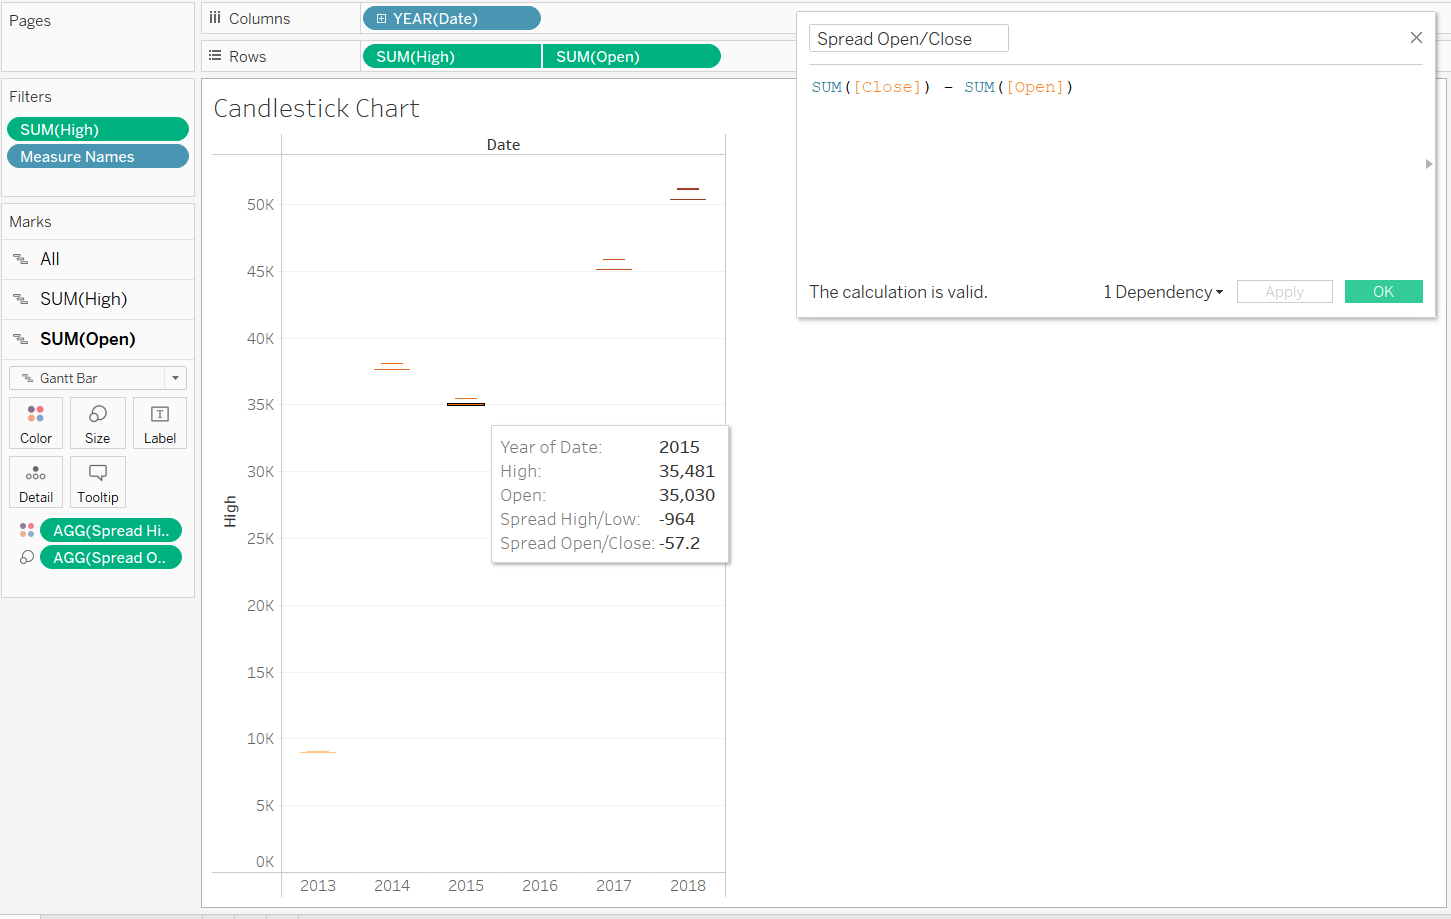
\includegraphics[scale=.20]{BDNen PTCK.png}
    \end{center}
    \caption{Biểu Đồ Nến Phân Tích Chứng Khoáng}
    \label{Biểu Đồ Nến Phân Tích Chứng Khoáng}
    \end{figure}
\end{center}
\end{frame}
 
 \begin{frame}{KẾT QUẢ NHẬN ĐƯỢC}
\begin{center}
    \begin{figure}[htp]
    \begin{center}
     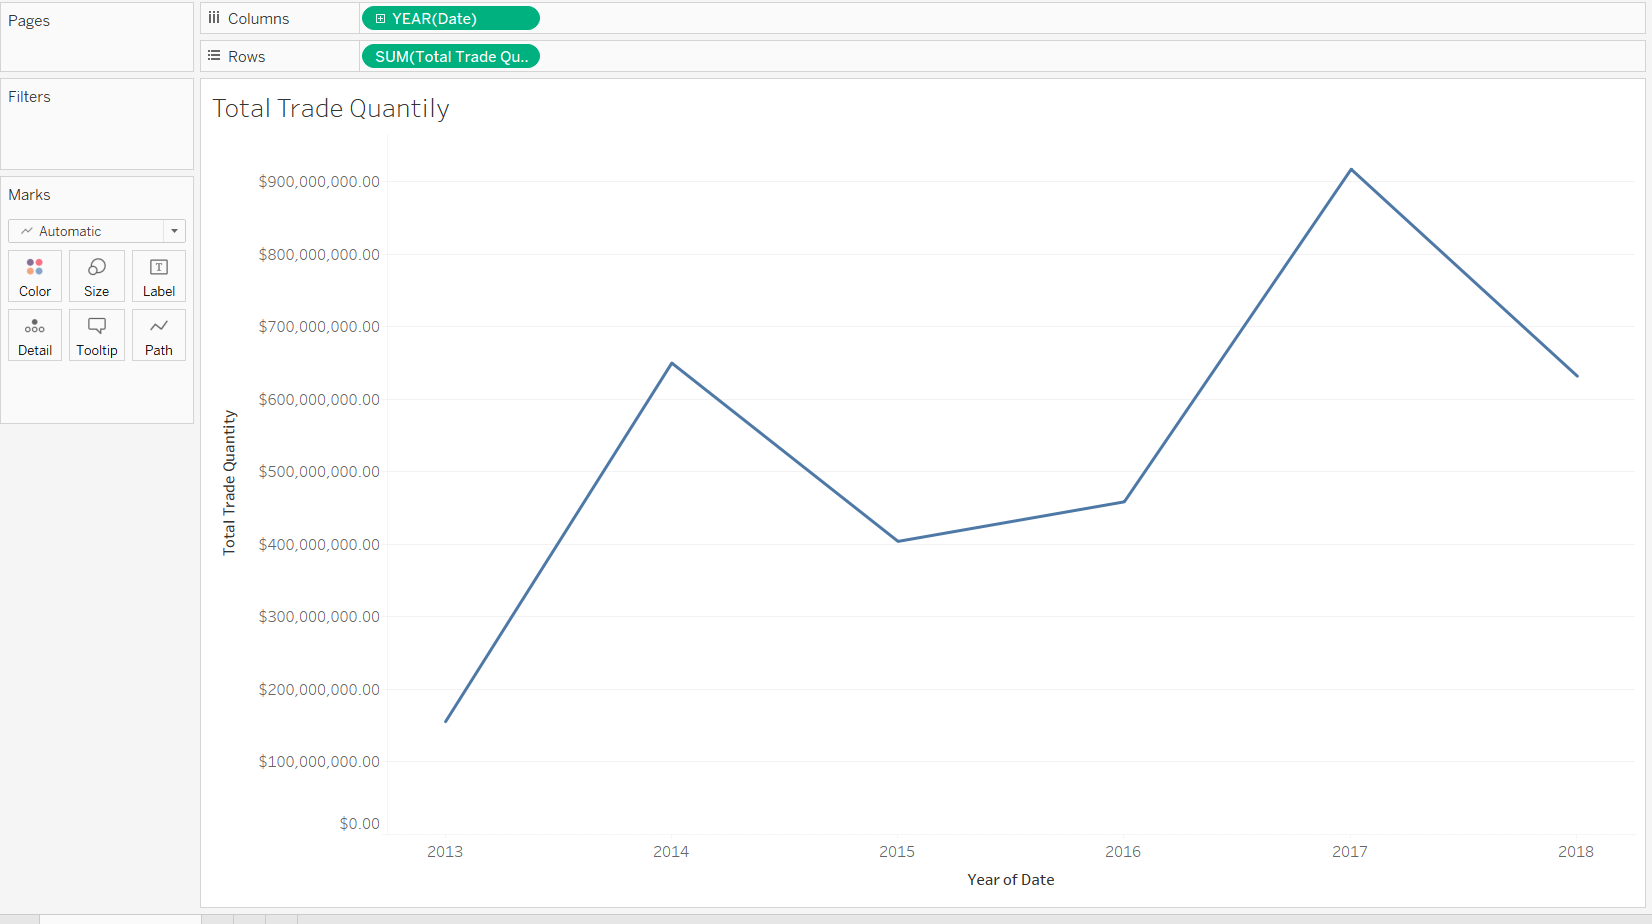
\includegraphics[scale=.20]{TLGD.png}
    \end{center}
    \caption{Tổng Lượng Giao Dịch Qua Từng Năm}
    \label{Tổng Lượng Giao Dịch Qua Từng Năm}
    \end{figure}
\end{center}
\end{frame}

\end{document}


